\appendix
\section{Appendix}

\subsection{Data}

%%%%%%%%%%%%%%%%%%%%%%%%%%%%%%%%%%%%%%%%%%%%%%%%%%%%%%%%%%%%%%%%%%%%%%%%%%%

\subsection{Probability, odds, and Shap values (log odds shifts): A brief explanation}

Many of us find it easiest to think of the chance of something occurring
as a probability. For example, there might be a probability of 10\% that
it will rain today. That is the same as saying there will be one rainy
day out of ten days for days with this given probability of rain.

In our stroke thrombolysis model, Shap values tell us how knowing
something particular about a patient (such as the patient
\emph{feature}, `Is their stroke caused by a clot or a bleed?') adjusts
our prediction of whether they will receive thrombolysis or not.

This is made a little more complicated for us because Shap is usually
reported as a \emph{log odds shift}. It is useful for us to see how
those relate to probabilities, and get a sense of how significant Shap
values in the range of 0.5 to 5 (or -0.5 to -5) are, as that is a common
range of Shap values that we will see in our models.

\subsubsection{Probability}

We will take the example that Shap reports that a model's base
probability prediction, before the contribution of features is 0.25, or
a 25\% probability of receiving thrombolysis; that is 1 in 4 patients
with this prediction would be expected to receive thrombolysis.

\subsubsection{Odds}

\emph{Probability} expresses the chance of something happening as the
number of positive occurrences as a fraction of all occurrences
(i.e.~the number of patients receiving thrombolysis as a fraction of the
total number of patients).

\emph{Odds} express the chance of something happening as the ratio of
the number of positive occurrences (i.e.~receiving thrombolysis) to the
number of negative occurrences (i.e.~\emph{not} receiving thrombolysis).

If we have probability prediction of 0.25 would receive thrombolysis,
that would mean 1 in 4 of those patients receive thrombolysis. Expressed
as odds, for every one patient that receives thrombolysis, three will
not. The odds are expressed as 1:3 or 1/3. This may also be calculated
as a decimal (1 divided by 3), 0.333.

Odds (O) and probability (P) may be converted with the following
equations:

\begin{enumerate}
\def\labelenumi{(\arabic{enumi})}
\item
  O = P / (1 - P)
\item
  P = O / (1 + O)
\end{enumerate}

\subsubsection{Shap values: Log odds shifts}

Here we will calculate the effect of Shap values, and try and build some
intuition on the size of effect Shap values of 0.5 to 5 give (we will
look at positive and negative Shap values).

Shap usually outputs the effect of a particular feature in how much it
shifts the odds. For reasons we will not go into here, that shift (which
is the `Shap value') is usually given in `log odds' (the logarithm of
the odds value). For the mathematically inclined, we use the natural log
(\emph{ln}).

Let's look at some Shap values (log odds) and see how much they change
the odds of receiving thrombolysis.

First we'll look at the shift in odds the Shap values give. This is
calculated as \emph{shift = exp(Shap)}

\begin{longtable}[]{@{}ll@{}}
\toprule
Shap (log odds) & Shift in odds (multiply original odds)\tabularnewline
\midrule
\endhead
0.5 & 1.65\tabularnewline
1 & 2.72\tabularnewline
2 & 7.39\tabularnewline
3 & 20.1\tabularnewline
4 & 54.6\tabularnewline
5 & 148\tabularnewline
\bottomrule
\end{longtable}

\emph{Positive Shap values: worked example}

Now let us work through an example of starting with a known baseline
\emph{probability} (before we consider what we know about a particular
patient feature), converting that to \emph{odds}, applying a Shap
\emph{log odds shift} for that particular feature, and converting back
to \emph{probability} after we have applied the influence of that
feature.

Here are the effects of those shifts on our baseline probability of
0.25.

\begin{longtable}[]{@{}llllll@{}}
\toprule
Starting P & Starting O & Shap & Shift (multiply O) & Shifted O &
Shifted P (\%)\tabularnewline
\midrule
\endhead
0.25 (25\%) & 0.333 & 0.5 & 1.65 & 0.550 & 0.3547
(35.5\%)\tabularnewline
0.25 (25\%) & 0.333 & 1 & 2.72 & 0.907 & 0.4754 (47.5\%)\tabularnewline
0.25 (25\%) & 0.333 & 2 & 7.39 & 2.46 & 0.7112 (71.1\%)\tabularnewline
0.25 (25\%) & 0.333 & 3 & 20.1 & 6.70 & 0.8700 (87.0\%)\tabularnewline
0.25 (25\%) & 0.333 & 4 & 54.6 & 18.2 & 0.9479 (94.8\%)\tabularnewline
0.25 (25\%) & 0.333 & 5 & 148 & 49.5 & 0.9802 (98.0\%)\tabularnewline
\bottomrule
\end{longtable}

So, for example, a Shap value of 0.5 for one particular feature tells us
that that particular feature in that patient shifts our expected
probability of that patient receiving thrombolysis from 25\% to 36\%. A
Shap value of 5 for the same feature would shift the probability of that
patient receiving thrombolysis up to 98\%.

\emph{Negative Shap values: worked example}

If we have a negative Shap value then odds are reduced (a Shap of -1
will lead to the odds being divided by 2.72, which is the same as
multiplying by 1/2.72, which is 0.3679):

\begin{longtable}[]{@{}llllll@{}}
\toprule
Starting P & Starting O & Shap & Shift (multiply O) & Shifted O &
Shifted P\tabularnewline
\midrule
\endhead
0.25 (25\%) & 0.333 & -0.5 & 0.6065 & 0.2022 & 0.1682
(16.8\%)\tabularnewline
0.25 (25\%) & 0.333 & -1 & 0.3679 & 0.1226 & 0.1092
(10.9\%)\tabularnewline
0.25 (25\%) & 0.333 & -2 & 0.1353 & 0.0451 & 0.0432
(4.32\%)\tabularnewline
0.25 (25\%) & 0.333 & -3 & 0.0498 & 0.0166 & 0.0163
(1.63\%)\tabularnewline
0.25 (25\%) & 0.333 & -4 & 0.0183 & 0.0061 & 0.0061
(0.61\%)\tabularnewline
0.25 (25\%) & 0.333 & -5 & 0.0067 & 0.0022 & 0.0022
(0.22\%)\tabularnewline
\bottomrule
\end{longtable}

So, for example, a Shap value of -0.5 for one particular feature tells
us that that particular feature in that patient shifts our expected
probability of that patient receiving thrombolysis from 25\% to 17\%. A
Shap value of 5 for the same feature would shift the probability of that
patient receiving thrombolysis down to 2\%.

\subsubsection{Observations about Shap values}

We begin to get some intuition on Shap values. A Shap value of 0.5 (or
-0.5) leads to a small, but still noticeable, change in probability.
Shap values of 5 or -5 have effectively pushed probabilities to one
extreme or the other.

%%%%%%%%%%%%%%%%%%%%%%%%%%%%%%%%%%%%%%%%%%%%%%%%%%%%%%%%%%%%%%%%%%%%%%%%%%%%%%%%%%%%%%%

\subsection{Feature selection}

A simplified model was created by using \emph{forward feature selection} where features were added in accordance to how much each one improved the Receiver Operating Characteristic (ROC) Area Under Curve (AUC). ROC AUC was measured using stratified k-fold validation (k=5). A model with all available 84 features had an ROC AUC of 0.922. A model with 10 features had an ROC AUC of 0.0.919.

The 10 features selected were:

\begin{itemize}
    \item \emph{Arrival-to-scan time}: Time from arrival at hospital to scan (mins)
    \item \emph{Infarction}: Stroke type (1 = infarction, 0 = haemorrhage)
    \item \emph{Stroke severity}: Stroke severity (NIHSS) on arrival
    \item \emph{Precise onset time}: Onset time type (1 = precise, 0 = best estimate)
    \item \emph{Prior disability level}: Disability level (modified Rankin Scale) before stroke
    \item \emph{Stroke team}: Stroke team attended
    \item \emph{Use of AF anticoagulants}: Use of atrial fibrillation anticoagulant (1 = Yes, 0 = No)
    \item \emph{Onset-to-arrival time}: Time from onset of stroke to arrival at hospital (mins)
    \item \emph{Onset during sleep}: Did stroke occur in sleep?
    \item \emph{Age}: Age (as middle of 5 year age bands)
\end{itemize}

\begin{figure}
\centering
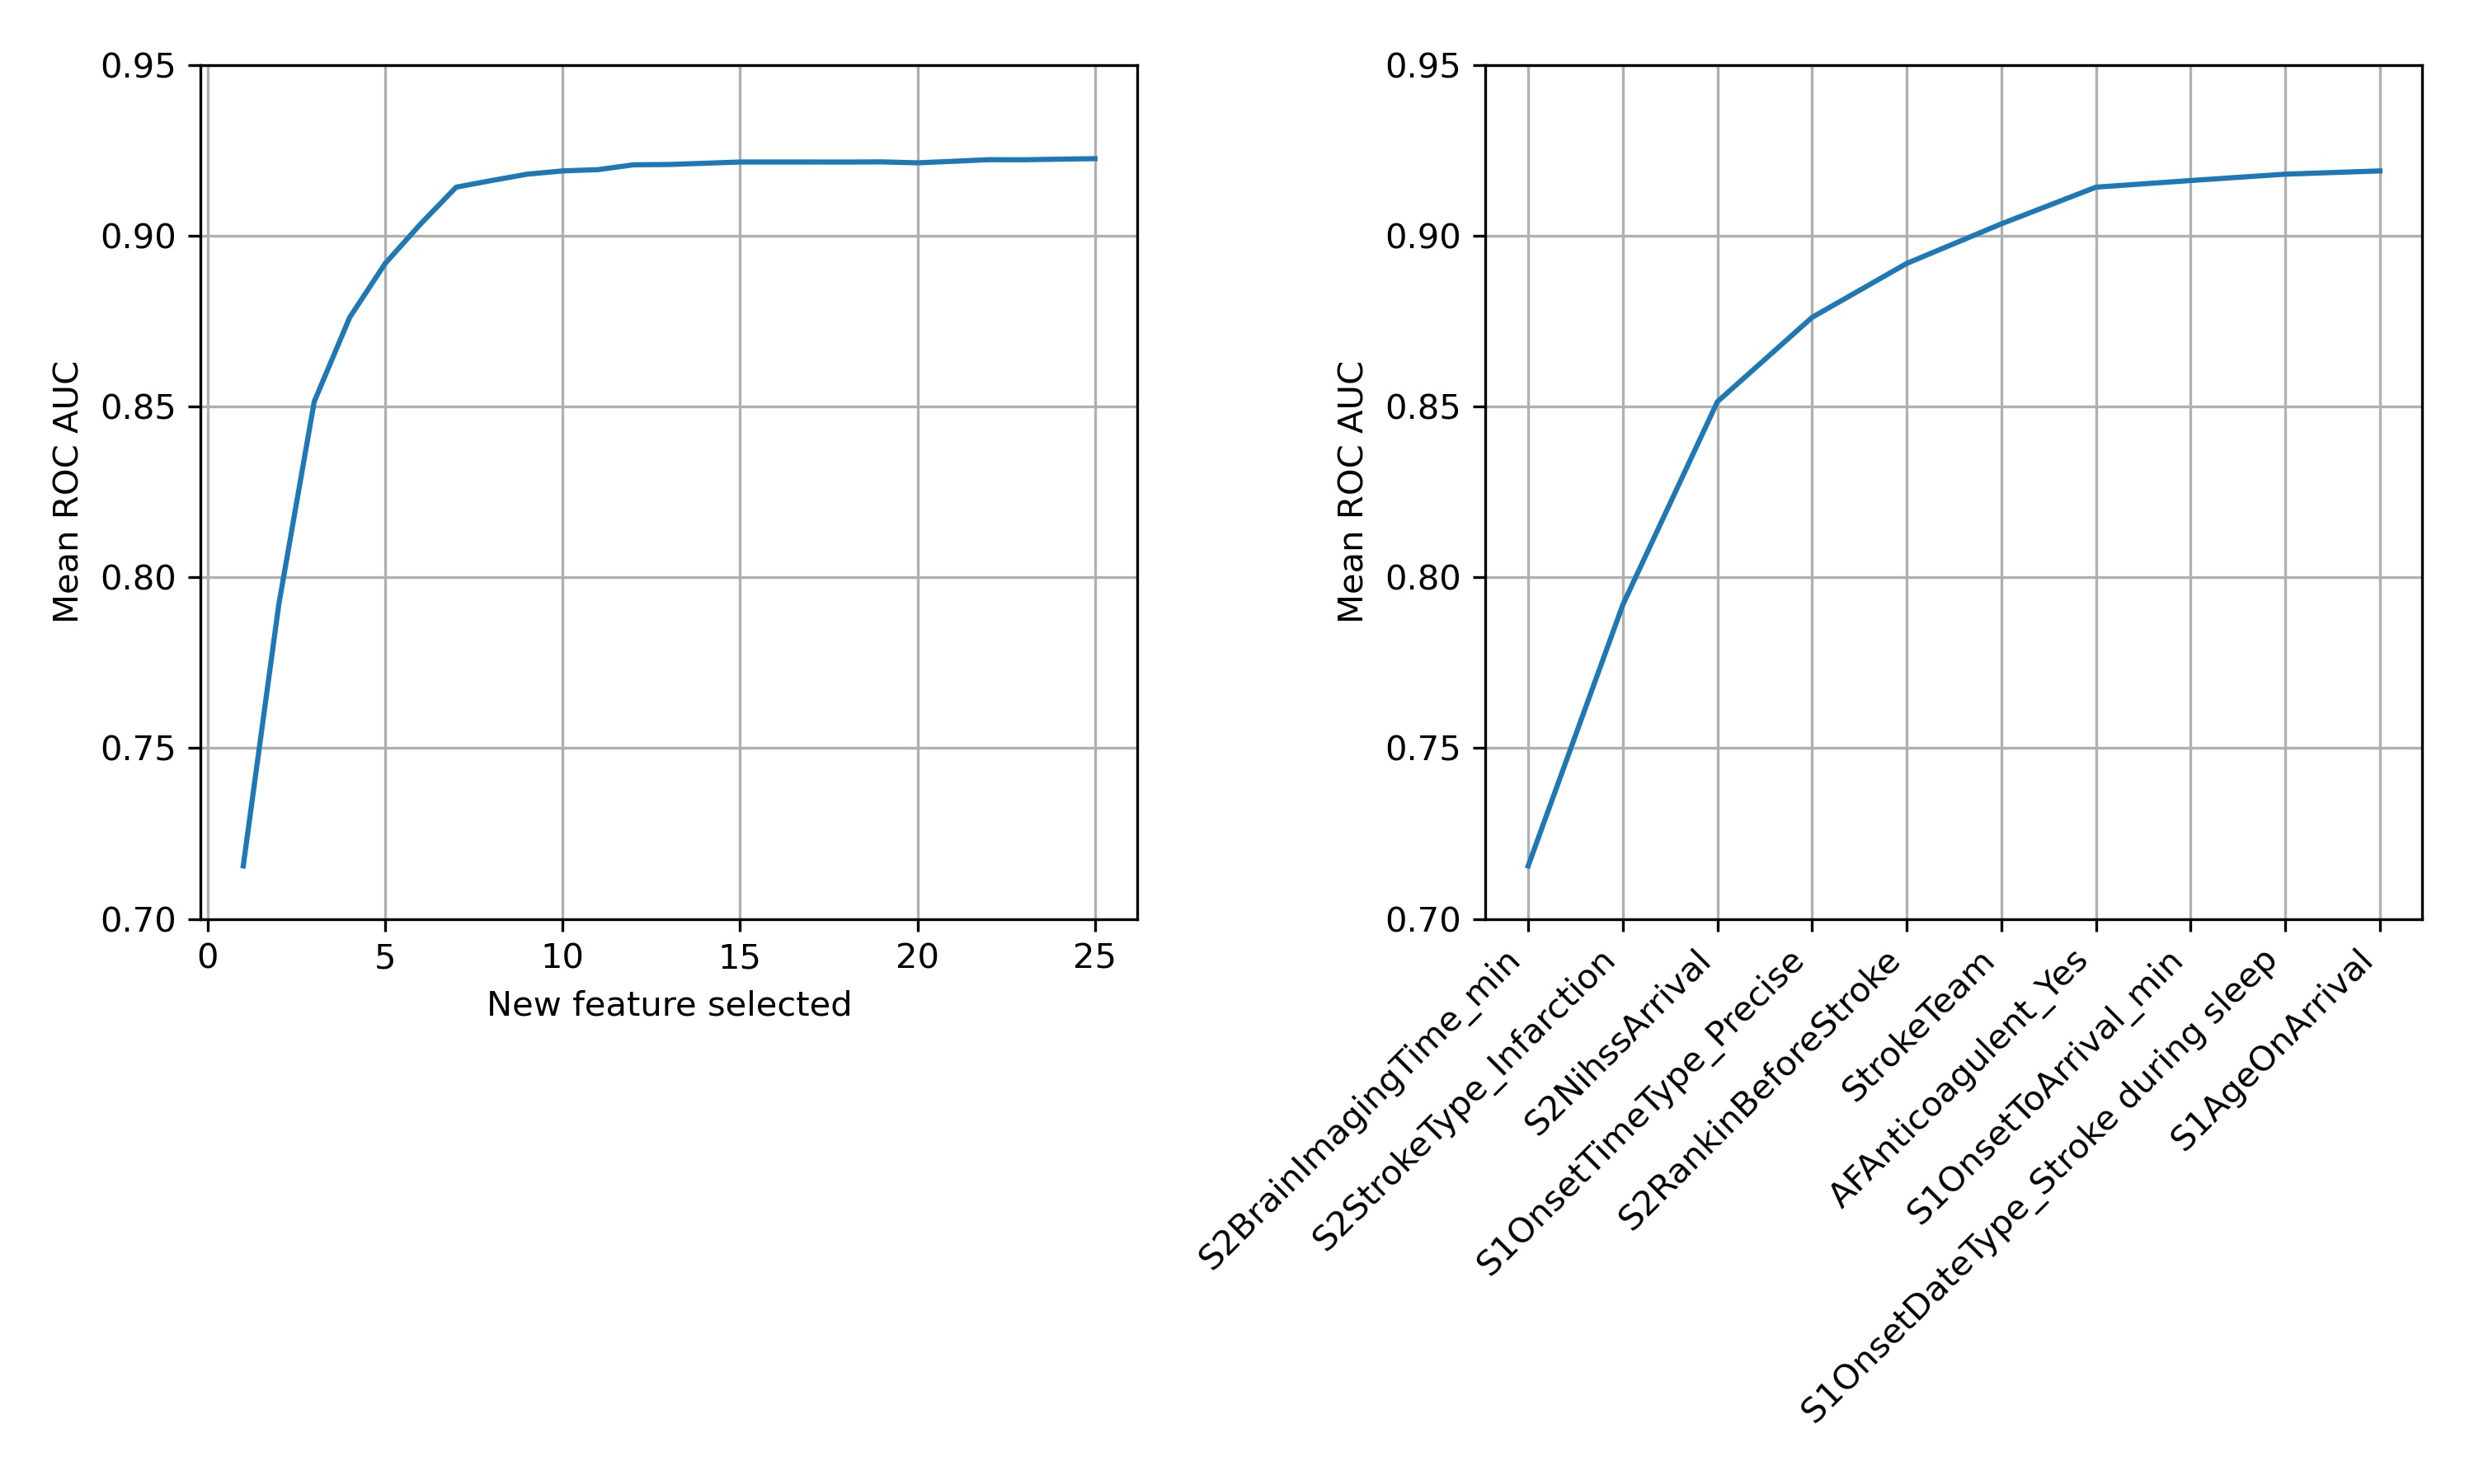
\includegraphics[width=1\textwidth]{./images/01_feature_selection}
\caption{The effect of progressively selecting more features on ROC AUC. Left: ROC AUC with selection of up to 25 features. Right: The first 10 selected features and the resulting ROC AUC.}
\label{fig:feature_selection}
\end{figure}

All results from this point forward will use the 10 feature model.

%%%%%%%%%%%%%%%%%%%%%%%%%%%%%%%%%%%%%%%%%%%%%%%%%%%%%%%%%%%%%%%%%%%%%%%%%%%%%%%%%%%%%%%

\subsection{Model accuracy}

The model was validated using stratified k-fold validation (k=5).
